\documentclass[runningheads]{llncs}

\usepackage[T1]{fontenc}
\usepackage{amsmath,amssymb}
\usepackage{array}
\usepackage{booktabs}
\usepackage{graphicx}
\usepackage{xcolor}
\usepackage{tikz}
\usetikzlibrary{arrows.meta,positioning,shapes.geometric}
\usepackage{hyperref}
\hypersetup{hidelinks}

\newcommand{\method}{ESV-Gap}
\newcommand{\statuseligible}{\texttt{automatically\_eligible}}
\newcommand{\hashbreak}[2]{\texttt{#1}\allowbreak\texttt{#2}}
\newcolumntype{L}[1]{>{\raggedright\arraybackslash}p{#1}}

\title{From Graph Signals to Evidence-Clear Research-Gap Candidates:\
Source-Disjoint Provenance and Multi-Mode Perturbation Testing}
\titlerunning{Evidence-Clear Research-Gap Candidates}

\author{Hoa Anh Le\inst{1} \and
Hoang Duc Nguyen\inst{1} \and
Khoa Ly Van Phan\inst{1} \and
Thanh Dinh Nguyen\inst{1}}
\authorrunning{H. A. Le et al.}

\institute{Department of Information Technology, FPT University, Ho Chi Minh City Campus, Vietnam\\
\email{\{hoalase181702, hoangndse181655, khoaplvse181656, thanhndse182854\}@fpt.edu.vn}\\[0.5em]
\textit{Faculty Supervisor:} Long Truong\\
Department of Software Engineering, FPT University, Ho Chi Minh City Campus, Vietnam\\
\email{longt5@fpt.edu.vn}}

\begin{document}
\setlength{\emergencystretch}{1em}
\maketitle

\begin{abstract}
Graph anomalies can generate research-gap candidates, but they do not establish novelty, importance, or absence from the literature. We present \method{}, a fail-closed triage stage that canonicalizes entity identity, requires source-disjoint provenance, tests relation-event deletion, paper dropout, and plausible edge addition, normalizes temporal activity, and routes coverage hits to review. Thresholds were selected on ten development seeds and frozen before a disjoint 50-seed test containing 800 candidates. The controlled test achieved precision, validator recall, and F1 of 1.000, compared with 0.250, 1.000, and 0.400 when every detector signal was retained; this verifies fixture behavior, not real-world gap quality. On an inherited 185-paper microservices-security snapshot, 256 signals were reduced to 40 review-required items, with none automatically eligible. A corrected live run for \emph{security of MongoDB}, configured with a 100-paper budget, collected 74 unique records, retained 53, extracted 643 relation events, and built a 578-node, 636-edge graph. The frozen gate reduced 128 signals to nine review-required items. One internal reviewer accepted eight of all nine post-gate items (88.9\%); separately, the same reviewer accepted 24 of 30 pre-gate ranked items (80.0\%). On the same corpus, a retrieval baseline produced 53 outputs and a per-abstract LLM baseline produced 159; lexical overlap with the graph candidates was 0.1239 and 0.1113. Because baseline outputs lack shared expert labels and the reviews are neither blinded nor independent, these live results establish workflow operability and preliminary reviewer disposition, not comparative effectiveness.

\keywords{Research-gap discovery \and Knowledge graphs \and Provenance \and Perturbation testing \and Evidence retrieval \and Systematic reviews.}
\end{abstract}

\section{Introduction}

Systematic reviews require transparent search, selection, and evidence accounting~\cite{page2021prisma}. Machine learning can accelerate screening and extraction, but automation should expose uncertainty and preserve human oversight~\cite{marshall2019automation,shneiderman2020hcai}. Research-gap discovery is especially sensitive: an omitted relation may reflect a genuinely under-studied question, an abstract-only corpus, an extraction false negative, an unresolved synonym, or a fragmented graph.

A recent preprint generated gap candidates from TransE link prediction, Louvain communities, and temporal decay~\cite{rahul2026dynamic}. Its eight-paper pilot reported 34 graph signals and a 90\% author accept-or-modify rate, while also reporting zero TransE outputs, 21 orphan communities, entity artefacts, and no independent baseline review. The useful insight is structural, but the epistemic interpretation must be narrower:

\begin{quote}
A graph anomaly is a candidate-generating signal; it is not a validated research gap.
\end{quote}

Our first ESV-Gap implementation enforced provenance, specificity, edge-dropout stability, direct-edge checks, and local lexical retrieval. Reviewer analysis exposed two important design defects. First, its weighted validation threshold was mathematically redundant: every candidate passing the hard rules already exceeded it. Second, a single two-edge path survived independent edge retention with expected probability $0.9^2=0.81$, above the 0.70 stability threshold. The revised method removes the score from the decision rule, requires source-disjoint path diversity, samples papers as evidence clusters, and tests plausible missing edges as well as deletions.

This paper makes four bounded contributions:

\begin{enumerate}
  \item an auditable evidence contract distinguishing \statuseligible{}, \texttt{review\_required}, and \texttt{rejected} without calling any automated output a confirmed gap;
  \item path-specific provenance and multi-mode perturbation testing that models false-positive extraction, correlated paper evidence, and plausible false-negative extraction;
  \item publication-normalized temporal detection with explicit right-censoring and a lexical candidate-coverage screen with acronym/synonym alternatives; and
  \item a disjoint-development, multi-signal benchmark with ablations and ranking metrics, a retrospective real-corpus diagnostic, and a corrected live MongoDB-security run with preliminary internal review and descriptive B1/B2 comparisons.
\end{enumerate}

The controlled results verify that the implementation rejects the planted artefacts. They do not establish detector recall, scientific novelty, usefulness, or real-world precision. Those claims require source-complete independent expert evaluation.

\section{Background and Related Work}

\subsection{Literature-based discovery and review automation}

Literature-based discovery predates modern language models. Swanson showed that separately published findings could be connected to form testable hypotheses~\cite{swanson1986fish}. Contemporary systematic-review automation addresses search, screening, extraction, and synthesis, but practical guidance emphasizes that readiness and risk differ by task~\cite{marshall2019automation}. ESV-Gap is closer to evidence triage than autonomous discovery: it reduces a candidate queue while preserving the sources and reasons needed by reviewers.

Scientific claim verification provides a relevant evaluation model. SciFact couples claims with evidence abstracts and rationales~\cite{wadden2020scifact}; SciFact-Open shows that systems evaluated on a small closed corpus can degrade substantially in open-domain retrieval~\cite{wadden2022scifactopen}. This motivates our asymmetric rule: a retrieval hit triggers review, while no hit is not proof of absence~\cite{altman1995absence}.

\subsection{Knowledge-graph uncertainty and provenance}

Knowledge graphs support extraction, completion, reasoning, and question answering~\cite{schneider2022decade}. TransE treats relations as translations in an embedding space~\cite{bordes2013transe}; uncertain KG embeddings instead retain graded fact confidence~\cite{chen2019ukge}. Generative extraction can introduce factual inconsistencies that propagate downstream~\cite{kim2026graphrefine}. Provenance therefore belongs to relation events, not only nodes. Our audit schema follows the spirit of PROV-O's entity, activity, and agent distinctions~\cite{lebo2013provo}: each event retains a paper, year, extraction identifier, confidence, and evidence span when available.

\subsection{Graph robustness and stability}

Louvain optimizes modularity and can expose communities~\cite{blondel2008fast}, but community structure may be unstable under sampling noise~\cite{karrer2008robustness,abbe2018community}. Stability selection similarly evaluates whether a result persists under resampling~\cite{meinshausen2010stability}. Our aim is narrower than either theory: candidate-level perturbation tests reveal dependence on particular edges, papers, or plausible missing bridges. A high survival rate is a robustness diagnostic, not a calibrated probability that the scientific claim is true.

\section{Problem Formulation}

Let a temporal literature graph be a directed multigraph
\begin{equation}
G=(V,E), \qquad e=(u,r,v,y,p,q,s),
\end{equation}
where $u,v\in V$ are typed entities, $r$ is a relation, $y$ a publication year, $p$ a paper identifier, $q$ an extraction confidence, and $s$ an evidence span. A detector $D_k$ maps $G$ to candidates $C_k$ of type missing link, orphan community, or temporal decline.

The validator does not estimate $\Pr(c\text{ is a real research gap})$. It computes an auditable decision
\begin{equation}
\delta(c)\in\{\texttt{automatically\_eligible},\texttt{review\_required},\texttt{rejected}\}.
\end{equation}
The first label means only that the automated evidence contract passed. Novelty, value, feasibility, and absence from source-complete literature remain human judgments. Detector recall concerns whether $D_k$ generated a relevant candidate; validator recall concerns whether $\delta$ retained a positive candidate already present in $C_k$; end-to-end recall combines both. Our controlled experiment estimates validator recall only.

\section{Method}

\subsection{Revised workflow}

\begin{figure}[t]
\centering
\resizebox{\textwidth}{!}{%
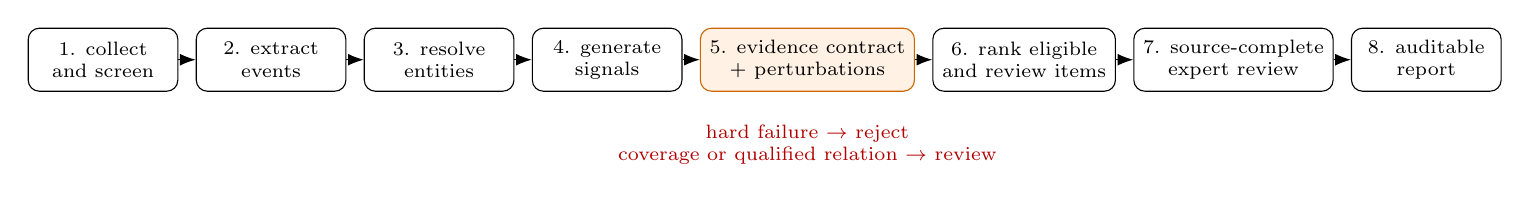
\begin{tikzpicture}[
  node distance=2.2mm,
  box/.style={draw,rounded corners,align=center,minimum height=8mm,minimum width=19mm,font=\scriptsize},
  gate/.style={box,draw=orange!80!black,fill=orange!10},
  arrow/.style={-{Latex[length=2mm]},thin}
]
\node[box] (collect) {1. collect\\and screen};
\node[box,right=of collect] (extract) {2. extract\\events};
\node[box,right=of extract] (resolve) {3. resolve\\entities};
\node[box,right=of resolve] (detect) {4. generate\\signals};
\node[gate,right=of detect] (validate) {5. evidence contract\\+ perturbations};
\node[box,right=of validate] (rank) {6. rank eligible\\and review items};
\node[box,right=of rank] (retrieve) {7. source-complete\\expert review};
\node[box,right=of retrieve] (report) {8. auditable\\report};
\foreach \a/\b in {collect/extract,extract/resolve,resolve/detect,detect/validate,validate/rank,rank/retrieve,retrieve/report}
  \draw[arrow] (\a) -- (\b);
\node[below=3mm of validate,font=\scriptsize,text=red!70!black,align=center] {hard failure $\rightarrow$ reject\\coverage or qualified relation $\rightarrow$ review};
\end{tikzpicture}}
\caption{Revised pipeline. Stage 5 separates candidate generation from claims about research gaps.}
\label{fig:pipeline}
\end{figure}

Figure~\ref{fig:pipeline} inserts the evidence contract before ranking. The implementation keeps parallel relation events instead of collapsing them into one adjacency, so paper-level sampling and temporal normalization remain possible. Every decision serializes metrics, thresholds, seeds, source-paper IDs, evidence paths, coverage hits, and all failed rules.

\subsection{Entity identity before graph topology}

Extractor type annotations are metadata rather than lexical identity. Before graph construction, Unicode is normalized, terminal suffixes such as \texttt{[METHOD]}, \texttt{[CONCEPT]}, and \texttt{[METRIC]} are removed, whitespace is collapsed, and labels that differ only by case share an identity key
\begin{equation}
\kappa(e)=\operatorname{casefold}(\operatorname{stripType}(\operatorname{NFKC}(e))).
\end{equation}
The first observed clean label is retained for display while type remains a node attribute. A missing-link pair with $\kappa(h)=\kappa(t)$ is discarded during graph construction and hard-rejected if encountered in legacy detector output. This prevents type or capitalization variants from creating artificial topology. For coverage retrieval, a terminal numeric protocol version also emits a versionless token, for example \texttt{OAuth2}$\mapsto\{\texttt{oauth2},\texttt{oauth}\}$.

\subsection{Specificity and path-specific provenance}

Let $T(e)$ be the non-stopword alphanumeric tokens in entity label $e$, and let $g(e)$ be the number that belong to a declared generic vocabulary. The explicit entity score is
\begin{equation}
q_s(e)=0.75\left(1-\frac{g(e)}{\max(|T(e)|,1)}\right)
+0.25\min\left(\frac{|T(e)|}{3},1\right),
\end{equation}
with score zero for an exact generic phrase. Candidate specificity $Q_s(c)$ is the mean over defining entities. The hard threshold is 0.55. This retains short specific labels such as TLS, JWT, and mTLS while rejecting phrases such as ``proposed framework.'' The vocabulary is configuration-visible and extensible.

For a missing-link candidate $(h,t)$, the validator enumerates simple paths of at most four edges and greedily selects paths that share neither an edge nor a source paper. Let $\Pi(c)$ be that selected set and $P(\pi)$ the papers on path $\pi$. Eligibility requires
\begin{equation}
|\Pi(c)|\geq 2,\qquad P(\pi_i)\cap P(\pi_j)=\varnothing\quad(i\neq j).
\end{equation}
Thus unrelated papers incident to $h$ or $t$ do not inflate support. For an orphan community, provenance counts only papers on internal edges. For a temporal candidate, it counts papers that mention the concept. A minimum of two paper IDs is mandatory. Research-group or shared-dataset independence cannot be inferred from the inherited metadata and remains a limitation.

\subsection{Isolation and normalized temporal activity}

For community members $M$, let $E_{\mathrm{in}}(M)$ be internal simple edges and $E_{\mathrm{cut}}(M)$ edges crossing to $V\setminus M$. Isolation is
\begin{equation}
I(M)=1-\frac{|E_{\mathrm{cut}}(M)|}{\max(|E_{\mathrm{in}}(M)|+|E_{\mathrm{cut}}(M)|,1)}.
\end{equation}
The detector and perturbation test use $I(M)\geq0.90$.

Raw relation-event counts confound topic activity with corpus growth. Let $n_{v,y}$ be the number of distinct screened papers mentioning concept $v$ in year $y$, and $N_y$ the total screened papers in that year. We use
\begin{equation}
a_{v,y}=\frac{n_{v,y}}{\max(N_y,1)},\qquad
d_v=1-\frac{\frac{1}{L}\sum_{y\in R}a_{v,y}}
{\frac{1}{L}\sum_{y\in H}a_{v,y}},
\end{equation}
where $H$ and $R$ are adjacent historical and recent windows of $L=2$ complete years. A signal requires $d_v\geq0.30$. The snapshot date is July 20, 2026, so 2026 is right-censored and excluded; the comparison ends in 2025.
The ratio is evaluated only when the historical mean is positive. When the historical mean is zero, both the detector and validation recomputation assign $d_v=0$: neither a zero-to-zero window nor new activity establishes decline.

\subsection{Candidate-coverage retrieval}

The local screen tokenizes titles and abstracts into lowercase alphanumeric tokens after applying the same type-suffix normalization. For every defining entity, the paper must cover at least
\begin{equation}
\max(1,\lceil0.60|T(e)|\rceil)
\end{equation}
tokens from either the canonical label or a declared acronym/synonym alternative. Relational candidates require two matched entity groups; temporal candidates require a post-peak match. The module is deliberately named candidate-coverage retrieval, not evidence closure: it does not resolve negation, direction, polarity, population, or study quality. A hit routes to review and never hard-rejects a candidate.

\subsection{Multi-mode perturbation stability}

For $B$ deterministic replicates, the defining signal is tested under three modes:

\begin{enumerate}
  \item \emph{relation-event deletion}: retain each event with probability $\rho$;
  \item \emph{paper dropout}: retain each paper with probability $\rho$ and jointly remove all its events; and
  \item \emph{plausible edge addition}: sample low-confidence, lexical-retrieval, or link-prediction edges supplied with the candidate.
\end{enumerate}

Let $I_{b,m}(c)$ indicate survival in replicate $b$ under mode $m$. We use the fail-closed score
\begin{equation}
Q_b(c)=\min_{m\in\mathcal{M}_{\mathrm{eval}}(c)}\frac{1}{B}\sum_{b=1}^{B}I_{b,m}(c).
\end{equation}
A missing-link signal survives when a short source-traceable path remains and no plausible direct edge is sampled. The two-path requirement is checked on the unperturbed graph, so a fragile single path cannot pass merely because $\rho^2$ exceeds the stability threshold. An orphan survives when $I(M)\geq0.90$; a temporal candidate survives when normalized decay remains at least 0.30. The development-selected configuration is $\rho=0.95$, $B=50$, and $Q_b\geq0.70$.

Here $\rho$ is a retention probability, so $\rho=0.95$ corresponds to 5\% expected deletion/dropout. Each candidate-relevant edge in the supplied \texttt{plausible\_edges} pool is sampled independently with probability 0.50 per replicate. Dictionary-form entries preserve endpoints, relation label, paper ID, year, and confidence; missing-link and orphan survival use endpoint topology without relation-direction matching. An empty or irrelevant pool is counted as an evaluated no-hit search only when \texttt{plausible\_edge\_search\_performed=true}; otherwise its mode value is JSON \texttt{null}, and fail-closed triage prevents automatic eligibility.

\subsection{Decision and ranking}

Insufficient path-specific provenance, specificity, path diversity, or stability, and any canonical self-link, is a hard rejection. A retrieved coverage hit, unavailable coverage corpus, unavailable plausible-edge stress test, or observed direct relation produces \texttt{review\_required}. An observed edge is not interpreted as proof that a broader research question is closed: reviewers must inspect relation type, polarity, context, outcome, date, and evidence strength. If no hard or review condition fires, the label is \statuseligible{}.

The previous acceptance threshold on a weighted validation score has been removed. For ordering only, available evidence metrics are combined as
\begin{equation}
R(c)=\frac{\sum_{j\in A(c)}w_jq_j(c)}{\sum_{j\in A(c)}w_j},
\end{equation}
where $A(c)$ contains applicable metrics. The default weights for provenance, specificity, path diversity, stability, and coverage clearance are, respectively,
\begin{equation}
(w_p,w_s,w_d,w_b,w_c)=(0.25,0.15,0.20,0.30,0.10).
\end{equation}
Changing $R(c)$ cannot change $\delta(c)$.

\section{Experimental Design}

\subsection{Research questions}

\textbf{RQ1:} Does the revised contract reject controlled artefacts across all three signal families? \textbf{RQ2:} Which validation components account for the improvement? \textbf{RQ3:} How sensitive are results to $\rho$, $B$, the stability threshold, and ranking weights? \textbf{RQ4:} How does the frozen gate change workload on the inherited real corpus? \textbf{RQ5:} How do graph candidates differ descriptively from retrieval and per-abstract LLM baselines on a corrected live corpus? \textbf{RQ6:} What does preliminary internal review show, and what evidence is still missing for a real-world effectiveness claim?

\subsection{Disjoint controlled benchmark}

The generator creates 16 candidates per seed: four positives and twelve negatives. Missing-link positives include two source-disjoint paths and short valid entity labels. Negatives include a qualified existing relation, generic labels, a single path, two topological paths sharing one source, a plausible omitted direct edge, synonym-only prior coverage, coverage hidden by a type suffix and protocol version, and a canonical self-link. Orphan cases include a stable multi-paper community, a one-study community, and a community vulnerable to plausible bridge addition. Temporal cases include normalized decline, raw-count decline with stable rate, and a false decline caused only by a partial final year.

Ten development seeds are reserved for a 48-cell sensitivity grid:
\begin{equation}
\begin{split}
\rho &\in \{0.70,0.80,0.90,0.95\},\qquad B\in\{50,100,200\},\\
\tau &\in \{0.70,0.80,0.90,0.95\}.
\end{split}
\end{equation}
Parameters are frozen before evaluation on 50 disjoint test seeds: 800 candidates, of which 200 are positive. Labels test planted artefact rejection, not scientific novelty.

For classification, $y=1$ denotes a planted evidence-sufficient candidate and $y=0$ a planted artefact or covered/qualified candidate. We set $\hat y=1$ only when the three-way gate returns \statuseligible{}; \texttt{review\_required} and \texttt{rejected} both map to $\hat y=0$. TP, FP, TN, and FN are therefore $(y,\hat y)=(1,1),(0,1),(0,0),(1,0)$. This evaluates automatic eligibility rather than possible later reviewer acceptance.

We compare retaining every signal with single-component gates, the hard contract without perturbation, the full contract without coverage retrieval, and the full contract. Ranking is evaluated with Precision@$k$, Recall@$k$, nDCG@$k$, and average precision for $k=200$. Detector score and evidence score receive the same candidate budget.

\subsection{Retrospective corpus diagnostic}

The inherited snapshot contains 185 microservices-security papers and 1,018 provenance-rich relation events spanning 2018--2026. Annual paper counts are 2, 3, 4, 13, 10, 23, 30, 68, and 32; the last value is partial and excluded from trend comparison. Events record the model identifier \path{ram/gemini-3.5-flash-low}, prompt version \path{triple-extraction-v2-provenance}, a prompt SHA-256, request timestamps, evidence spans, and paper IDs. Canonicalization reduces the graph from 1,149 raw labels to 1,130 entity nodes; the resulting multigraph contains 1,018 events and 176 weak components.

A reproducible integrity audit found 185 unique paper IDs, abstracts for every record, 184 DOI-bearing records, and a Semantic Scholar CorpusId for all 185. All 184 DOI strings returned a resolver redirect on August 5, 2026. Every relation event maps to a corpus paper and has an evidence quote; 989 of 1,018 quotes (97.15\%) are exact case-insensitive substrings of the recorded source abstract. The remaining 29 unmatched quotes are retained as auditable extraction risks rather than silently discarded.

The preserved snapshot does not contain its original database query, retrieval ledger, deduplication counts, or independent screening agreement. It records a lexical-first-pass screening reason for each retained paper. Consequently, this experiment is a retrospective diagnostic, not a reproducible PRISMA corpus construction and not an independent replication. We run deterministic common-neighbour missing-link generation (top 50), fixed-seed Louvain, and normalized temporal decay. The lightweight missing-link generator exercises the signal family on CPU but is not presented as a tuned TransE replacement.

\subsection{Corrected live MongoDB-security execution}

On August 6, 2026, we reran the deployed Streamlit path with the topic \emph{security of MongoDB} and a maximum collection budget of 100 papers. The immutable directory \path{runs/security_of_mongodb_20260806_135447} preserves 74 unique Semantic Scholar records returned across five queries, 53 abstracts retained by the topic-conditioned screener, all per-paper extraction files, the graph, detector and ranking outputs, an internal review record, and both baseline outputs. The 100-paper value is a ceiling rather than an achieved sample size. All retained records were published from 2020 through 2025; the annual counts were 2, 3, 4, 11, 7, and 26.

The Groq-hosted \path{llama-3.1-8b-instant} model was used for screening, extraction, and generation. Missing-link generation used the deterministic common-neighbour fallback because PyKEEN was unavailable. We define B1 as the Mulla-style retrieval baseline: for each paper, the three most similar abstracts are retrieved and the model generates one structured \texttt{REMAINING\_GAPS} field. Because \path{sentence_transformers} was unavailable, all 53 B1 cases used TF--IDF cosine retrieval. B2 is a no-retrieval per-abstract prompt that requests three gaps. Both baselines use the same 53-paper corpus and model. We compare output count, uniqueness, mean length, and corpus-level token-set Jaccard overlap. These are descriptive measures, not accuracy metrics.

One reviewer identified in the artifact as \path{author_internal} assessed two separate queues using Accept, Reject, Modify, or Pending: the 30 graph candidates ranked before gate application and all nine post-gate \texttt{review\_required} candidates. The queues overlap by one item. Neither review was blinded, neither included B1/B2 outputs, and neither contains a second reviewer, adjudication, or item-level rationale. They are therefore author-internal disposition records and do not replace the independent expert protocol.

The deployed path represented by this run executes collection, screening, extraction, graph construction, detection, scoring, and visualization, but it does not invoke the separate \path{validate_all_gaps} stage used in the frozen evidence-contract experiments. Accordingly, the top 30 are detector-ranked candidates with \texttt{validation=null}, not \statuseligible{} decisions. The UI review labels record reviewer disposition toward those candidates; they do not certify that the frozen gate was passed.

\section{Results}

\subsection{Controlled classification and ablation}

\begin{table}[t]
\caption{Held-out controlled test (800 candidates; 200 positives). Recall is validator recall conditional on candidate generation.}
\label{tab:controlled}
\centering
\begin{tabular}{lrrrrrrr}
\toprule
Method & TP & FP & TN & FN & Prec. & Rec. & F1\\
\midrule
Retain every signal & 200 & 600 & 0 & 0 & .250 & 1.000 & .400\\
Full evidence contract & 200 & 0 & 600 & 0 & 1.000 & 1.000 & 1.000\\
\bottomrule
\end{tabular}
\end{table}

Table~\ref{tab:controlled} shows that the full contract removed all 600 planted negatives without losing a planted positive. The false positives therefore fell from 600 to zero in this controlled test. Results were also perfect within missing-link (100 positives, 400 negatives), orphan (50, 100), and temporal (50, 100) strata. The zero-width 95\% interval across deterministic seed-level F1 values is $[1.000,1.000]$; this reflects identical fixture difficulty across seeds, not population uncertainty.

\begin{table}[t]
\caption{Ablation on the held-out test.}
\label{tab:ablation}
\centering
\begin{tabular}{lrrrr}
\toprule
Configuration & FP & Precision & Recall & F1\\
\midrule
Provenance only & 550 & .267 & 1.000 & .421\\
Specificity only & 550 & .267 & 1.000 & .421\\
Path diversity only & 500 & .286 & 1.000 & .444\\
Perturbation only & 350 & .364 & 1.000 & .533\\
Hard contract, no perturbation & 300 & .400 & 1.000 & .571\\
Full, no coverage retrieval & 100 & .667 & 1.000 & .800\\
Full evidence contract & 0 & 1.000 & 1.000 & 1.000\\
\bottomrule
\end{tabular}
\end{table}

Table~\ref{tab:ablation} shows that no single rule explains the result. Coverage retrieval removes the remaining synonym-coverage negative, while source-disjoint paths and multi-mode perturbations address different dependence failures.

\subsection{Sensitivity and ranking}

Across the 48 development configurations, F1 ranged from 0.462 to 1.000; seven cells were perfect. Mean F1 rose from 0.549 at $\rho=0.70$ to 0.940 at $\rho=0.95$. Increasing $B$ from 50 to 200 changed mean F1 from 0.722 to 0.752, while increasing the threshold from 0.70 to 0.95 reduced mean F1 from 0.873 to 0.625. We selected the lowest-cost perfect development configuration, $(\rho,B,\tau)=(0.95,50,0.70)$, before opening the test results.

At the matched budget $k=200$, detector-score ranking placed no positive in the first 200 positions and achieved average precision 0.153. Evidence-score ranking achieved Precision@200 and Recall@200 of 0.770, nDCG@200 of 0.816, and average precision of 0.906. Equal, provenance-heavy, and path-heavy schemes shared nDCG@200 of 0.816; stability-heavy obtained 0.815 and specificity-heavy 0.704. Hard decision reasons such as canonical self-link are intentionally not encoded as another weighted acceptance threshold, so ranking is useful but imperfect.

\subsection{Real-corpus triage}

\begin{table}[t]
\caption{Frozen-gate outcome on the 185-paper snapshot.}
\label{tab:real}
\centering
\begin{tabular}{lrrrr}
\toprule
Signal & Raw & Eligible & Review & Reject\\
\midrule
Missing link & 50 & 0 & 14 & 36\\
Orphan community & 194 & 0 & 17 & 177\\
Temporal decay & 12 & 0 & 9 & 3\\
\midrule
Total & 256 & 0 & 40 & 216\\
\bottomrule
\end{tabular}
\end{table}

Table~\ref{tab:real} shows a reduction from 256 detector signals to 40 review-required items, an 84.4\% workload reduction before source-complete review. Candidate-coverage retrieval fired for 245 signals; 177 lacked two paper IDs, 36 missing-link candidates lacked two source-disjoint paths, 18 were unstable, and four were underspecified. Reasons overlap because every failure is retained.

No real-corpus item is \statuseligible{}. The five items previously assigned that label were artifacts of entity identity or coverage tokenization. After canonicalization, Scalability \texttt{[CONCEPT]}--scalability \texttt{[METRIC]} collapses to a self-link and is not generated; JWT--OAuth, API Gateway--Microservices, Latency--Microservices, and Microservices--throughput have 9, 25, 21, and 5 local co-mention hits and therefore require review. This correction is fail-closed: it does not assert that co-mention closes a scientific question.

\subsection{Observed live-run outputs}

\begin{table}[t]
\caption{Observed outputs of the corrected MongoDB-security run (collection budget 100).}
\label{tab:live}
\centering
\begin{tabular}{L{6.0cm}r}
\toprule
Artifact or stage & Observed value\\
\midrule
Unique records collected and screened & 74\\
Abstracts retained & 53 (71.6\%)\\
Non-empty extraction outputs & 53 of 53\\
Extracted relation events & 643\\
Knowledge graph & 578 nodes; 636 edges; 61 components\\
Raw signals & 128 (50 missing; 71 orphan; 7 temporal)\\
Ranked top-30 & 4 missing; 25 orphan; 1 temporal\\
Normalized score range & 0.9936--1.0000\\
\bottomrule
\end{tabular}
\end{table}

Table~\ref{tab:live} reports artifact counts rather than projected values. Extraction produced 643 events; graph-construction filtering retained 636 edges after controlled-relation and self-loop checks. The graph contained 61 weak components, which is consistent with the dominance of orphan-community signals. The ranker's narrow normalized score range is a within-run min--max effect and is neither a calibrated novelty probability nor evidence that the candidates are nearly equivalent in scientific value.

\begin{table}[t]
\caption{Descriptive comparison on the same 53-paper corpus. B1 uses top-3 TF--IDF retrieval; B2 uses no retrieval.}
\label{tab:baselines}
\centering
\begin{tabular}{L{3.0cm}rrrr}
\toprule
Method & Outputs & Unique & Mean words & Jaccard vs KG\\
\midrule
KG candidate ranker & 30 & 30 & 27.6 & 1.0000\\
B1: retrieval + LLM & 53 & 53 & 67.2 & 0.1239\\
B2: per-abstract LLM & 159 & 159 & 28.9 & 0.1113\\
\bottomrule
\end{tabular}
\end{table}

B1 generated one structured remaining-gap output for every retained paper, whereas B2 generated three outputs per paper. B1 and B2 had a token-set Jaccard overlap of 0.3333. The lower overlap between either baseline and the graph candidates indicates different vocabulary and granularity, not superiority. No shared expert labels, precision, recall, or ranking judgment are available for B1/B2, and the graph scores are not comparable to language-model likelihoods.

\begin{table}[t]
\caption{Preliminary author-internal review of the ranked graph candidates.}
\label{tab:mongodb-review}
\centering
\begin{tabular}{lrrrrr}
\toprule
Signal & Shown & Accept & Modify & Reject & Pending\\
\midrule
Missing link & 4 & 0 & 0 & 4 & 0\\
Orphan community & 25 & 23 & 0 & 2 & 0\\
Temporal decay & 1 & 1 & 0 & 0 & 0\\
\midrule
Total & 30 & 24 & 0 & 6 & 0\\
\bottomrule
\end{tabular}
\end{table}

All 30 items in Table~\ref{tab:mongodb-review} received a decision: 24 were accepted (80.0\%) and six rejected. No item remained Modify or Pending. All four missing-link candidates were rejected; 23 of 25 orphan-community candidates and the single temporal candidate were accepted. These figures measure one internal reviewer's disposition toward the displayed queue. They do not estimate population precision or inter-rater reliability.

\begin{table}[t]
\caption{Complete author-internal review of the post-gate queue.}
\label{tab:postgate-review}
\centering
\begin{tabular}{lrrr}
\toprule
Signal & Shown & Accept & Reject\\
\midrule
Orphan community & 3 & 3 & 0\\
Temporal decay & 6 & 5 & 1\\
\midrule
Total & 9 & 8 & 1\\
\bottomrule
\end{tabular}
\end{table}

All nine post-gate items received a decision: eight were accepted (88.9\%) and one was rejected, with no Modify or Pending label. The rejected item was the \emph{Cloud infrastructure} temporal signal. Here ``Accept'' means retain an uncertainty-routed candidate for follow-up; it does not establish novelty or a source-complete literature gap.

\subsection{Three audit case studies}

\begin{table}[h]
\caption{Representative audit outcomes.}
\label{tab:cases}
\centering
\begin{tabular}{L{2.3cm}L{4.0cm}L{5.0cm}}
\toprule
Outcome & Candidate & Auditable reason\\
\midrule
Rejected & AWS API Gateway--Security & Only one source-disjoint path; 28 local co-mentions cannot repair insufficient provenance.\\
Review required & Docker--Kubernetes & Hard evidence checks pass, but five screened abstracts co-mention the concepts.\\
Removed self-link & Scalability variants & Type suffixes and case are metadata; both labels canonicalize to the same entity.\\
Review required & JWT--OAuth & Two source-disjoint paths pass, but nine local abstracts co-mention the normalized labels.\\
\bottomrule
\end{tabular}
\end{table}

\section{Preliminary Review and Expert Evaluation Protocol}

The MongoDB-security run includes complete author-internal decisions for the nine post-gate candidates and for the 30 pre-gate ranked candidates. These records supply disposition counts and verify that the review interface persists decisions, but they lack blinding, independent reviewers, source-complete searches, written rationales, and baseline judgments. The cohorts overlap by one item and are not independent samples. We therefore report them separately from the planned effectiveness study and do not use either acceptance rate to estimate expert precision.

To make an independent study executable, the artifact also creates a 70-item blinded packet for the inherited microservices snapshot: all 40 non-rejected items plus a deterministic stratified sample of 30 rejected items. At least three domain experts should independently rate source support, novelty after source-complete retrieval, importance, actionability, feasibility, already-addressed status, extraction error, and review time. Reviewers should be blinded to system status and receive identical full-text and citation-neighbourhood bundles. Budget-matched B1, B2, and detector-score candidates should be mixed into the packet. The analysis should report expert precision, an estimated false-negative rate from rejected items, usefulness, time per candidate, and Krippendorff's alpha or Fleiss' kappa. Until that study is completed, the real-corpus evidence supports operability, auditability, and preliminary reviewer disposition only.

\section{Discussion}

The first conceptual correction is that entity identity precedes topology. Treating \texttt{[METHOD]} or \texttt{[METRIC]} as lexical content created artificial nodes and caused the coverage screen to require words that never belonged to the scientific concept. The second is the unit of evidence. A node may have many incident papers while the candidate relation depends on one source. Source-disjoint paths expose that dependence. Paper dropout then respects correlation among events extracted from the same document. Plausible edge addition tests the opposite failure mode from deletion: an apparent missing relation or orphan community may result from extraction false negatives.

The revised temporal rule also changes interpretation. The inherited corpus grew sharply in 2025 and contains only a partial 2026. Normalizing by $N_y$ and excluding 2026 prevents corpus growth and right-censoring from being mistaken for topic decline. The remaining 12 signals all require expert interpretation.

The corrected live run separates software operability from scientific validity. It verifies collection, screening, extraction, graph construction, fallback detection, frozen-gate evaluation, ranking, review persistence, and both baseline paths on a topic-conditioned 53-paper corpus. The post-gate 88.9\% and pre-gate 80.0\% acceptance rates are reviewer-disposition summaries, not precision estimates: both reflect the same unblinded internal reviewer and do not replace independent expert evaluation. The low Jaccard overlap against B1 and B2 shows that the aggregate token sets differ; it motivates, but does not substitute for, shared-label accuracy comparisons.

Perfect controlled performance should invite caution. The revised generator is more varied than direct rule-copy negatives, covers all signal families, and is separated from development seeds, but it remains authored with knowledge of the intended evidence contract. It tests implementation behavior and known failure modes, not generalization to naturally occurring research gaps. Likewise, the evidence score's perfect controlled ranking is not a real-world ranking result.

\section{Limitations and Threats to Validity}

The inherited real corpus is abstract-only, single-domain, retrospectively collected, and missing its original search and screening ledger. Twenty-nine evidence quotes are not verbatim substrings of their recorded abstracts and require source inspection. The corrected live run retained 53 of 74 collected papers and supplied a topic-focused corpus for an operational comparison, but it used a single Groq-hosted 8B model for all LLM stages, TF--IDF fallback for B1 retrieval, and a common-neighbour fallback for link prediction. The displayed top 30 were ranked before the separate frozen gate and cannot be interpreted as having passed it. The same unblinded author reviewed those 30 and all nine post-gate candidates, with one overlapping item, no second reviewer or adjudication, and no item-level rationales; B1/B2 outputs were not included in either packet. Candidate-coverage retrieval remains lexical even with aliases and version normalization; it does not verify relation direction, polarity, population, method, or outcome. Plausible additions are available only when an upstream retriever supplies them. Entity merge/split perturbation, relation-label corruption, extraction-model reruns, full-text retrieval, and citation chasing remain future work.

Distinct papers are not necessarily independent studies: author groups, datasets, and paper extensions are not modeled. The greedy path selector is deterministic but not guaranteed to find the maximum source-disjoint set. Louvain remains resolution-sensitive. Perturbation thresholds are development choices, not calibrated probabilities. The real missing-link generator is a deterministic common-neighbour baseline rather than TransE. Although both internal review queues are complete, there are no independent source-verified labels and no labels for B1/B2. Real precision, recall, usefulness, time savings, detector recall, and workflow recall therefore remain unknown. The controlled benchmark's perfect result must not be read as evidence that the system discovers true gaps perfectly.

\section{Reproducibility and Artifact Availability}

The code emits \path{evidence_clear_candidates.json}, \path{review_required_gaps.json}, and \path{gap_validation_audit.json}. The controlled and real reports preserve every decision and perturbation-mode survival rate. The separate \path{corpus_integrity_audit.json} records identifier, DOI-resolution, provenance, and verbatim-evidence checks. The blinded expert packet contains blank rating fields; no synthetic judgments are inserted. The live run separately preserves \path{expert_reviews.json}, \path{post_gate_expert_reviews.json}, \path{comparison_metrics.json}, and both baseline output files.

\begin{table}[t]
\caption{Artifact contract at the time of this revision.}
\label{tab:artifact}
\centering
\begin{tabular}{L{3.2cm}L{8.0cm}}
\toprule
Field & Value\\
\midrule
Repository & \href{https://github.com/Khoa-Hoa-Technology-Solution-Company/research-paper-gap}{GitHub: Khoa-Hoa-Technology-Solution-Company/research-paper-gap}\\
Source snapshot & Curated in \path{esv-gap-final-20260810-r1.zip}; 43 files are covered by \path{MANIFEST.sha256}.\\
Archive SHA-256 & \hashbreak{c6e3d3daf7959598b68b386d39fb8af4}{126a1d98e7d314e64b239cd07483c835}.\\
Runtime & CPython 3.14.6; \path{requirements-experiments.lock}.\\
Triple snapshot SHA-256 & \hashbreak{2dc2ba9adba91f1f5ba8d49c0efe3ef}{56e8a906289e606242b10dcf866760253}.\\
Corpus snapshot SHA-256 & \hashbreak{413d757a467f0e67166b4a7d83a9ed296}{c4414406f3ccf0aa6ddc323a4bc13a2}.\\
Live run & \path{security_of_mongodb_20260806_135447}; 74 collected, 53 retained, 643 relation events, 128 raw detector signals, and 30 ranked.\\
Commands & Exact test, benchmark, corpus, review-packet, hash, and LaTeX commands are in \path{paper_v2/REPRODUCIBILITY.md}.\\
License & No license is declared in the inherited repository; no reuse rights are asserted here.\\
\bottomrule
\end{tabular}
\end{table}

The benchmark report SHA-256 is
\hashbreak{9796cbcdd08b7a13e60b8a37eea8cbd5}{a8418feb2c845a5e852fe5e6ecb2e4fe}; the real diagnostic report SHA-256 is
\hashbreak{0457dd177ad56e2a809cad41f4eb3acc}{d4430a0acee69be7338f983885217c26}; the corpus-integrity audit SHA-256 is
\hashbreak{dc1fc3a8713a45f21470a368e9a82957}{8512b3a7f4b770c727bcade962a54a10}. The live-run SHA-256 values are:
\begin{itemize}
  \item filtered corpus: \texttt{1f47c496466ce241b72330c9a80ceaf3}\linebreak
    \texttt{84de683f8af49b98bc30b75e7d244853};
  \item extracted triples: \texttt{bf17038593413d26c60b1a8d781ed1d5}\linebreak
    \texttt{ad580722c8d93542be2cba4b176a0386};
  \item raw detector output: \texttt{3af4d23f82ab1e3c7200825743ecce9b}\linebreak
    \texttt{2f418bfcdc4ff6c6591997ce4cc51d12}; and
  \item ranked top-30 output: \texttt{9cd92844fb48d24534b484838c3b1c49}\linebreak
    \texttt{46eb6bb737b7edeb48d3657c58d506e2};
  \item pre-gate internal review: \texttt{02a355a757f67f7af1aef9b08c13363d}\linebreak
    \texttt{7a73c8d5f285f7d1f1252f5671cbec64};
  \item post-gate internal review: \texttt{390b91827507a27383a3c972b90e81425}\linebreak
    \texttt{cbd44f921b2ac5cdc87e791b84e18aa}; and
  \item comparison metrics: \texttt{ecee805edf656c6bb043be39846e50a7}\linebreak
    \texttt{eb5e729ed359a03908c2a712cadfe25e}.
  \item frozen live gate report: \texttt{06eadc23301857b636378cdd8a0e236b}\linebreak
    \texttt{08df94937a688a9f91e44b3564e2f46d}.
\end{itemize}
The archived command is \path{python reproduce_frozen_validation.py --config frozen_validation_config.yaml}; it reproduces the 0/9/119 eligible/review/reject summary without network access. These hashes will change if the reports are regenerated under modified code or configuration.

\section{Conclusion}

\method{} treats graph anomalies as hypotheses and makes the evidence contract explicit. The revision canonicalizes identity before topology, rejects canonical self-links, requires source-disjoint evidence paths, samples whole papers, tests plausible edge additions, normalizes temporal activity, and excludes a partial final year. On an 800-candidate controlled test it rejected every planted artefact, but that result establishes only controlled implementation validity. On a 185-paper retrospective snapshot it reduced 256 signals to 40 review-required candidates and automatically accepted none. A corrected live run on \emph{security of MongoDB} collected 74 records, retained 53, extracted 643 relation events, and built a 578-node graph. The frozen gate reduced 128 signals to nine review-required items; one internal reviewer accepted eight of those nine (88.9\%) and, separately, 24 of 30 pre-gate ranked items (80.0\%). On the same corpus, retrieval and per-abstract LLM baselines produced 53 and 159 outputs with Jaccard overlaps of 0.1239 and 0.1113 against the graph candidates. Because no shared expert labels exist for the baselines and the reviews were neither blinded nor independent, the live results support workflow operability and preliminary disposition, not comparative effectiveness. A preregistered, source-complete, multi-domain expert study evaluating both retained and rejected candidates is required before making effectiveness claims.

\begin{credits}
\subsubsection{Acknowledgements}
The authors thank FPT University for supporting this research.

\subsubsection{Disclosure of Interests}
The authors have no competing interests to declare that are relevant to the content of this article.
\end{credits}

\bibliographystyle{splncs04}
\bibliography{references}

\end{document}
